% Options for packages loaded elsewhere
\PassOptionsToPackage{unicode}{hyperref}
\PassOptionsToPackage{hyphens}{url}
\PassOptionsToPackage{dvipsnames,svgnames,x11names}{xcolor}
%
\documentclass[
  letterpaper,
  DIV=11,
  numbers=noendperiod]{scrartcl}

\usepackage{amsmath,amssymb}
\usepackage{lmodern}
\usepackage{iftex}
\ifPDFTeX
  \usepackage[T1]{fontenc}
  \usepackage[utf8]{inputenc}
  \usepackage{textcomp} % provide euro and other symbols
\else % if luatex or xetex
  \usepackage{unicode-math}
  \defaultfontfeatures{Scale=MatchLowercase}
  \defaultfontfeatures[\rmfamily]{Ligatures=TeX,Scale=1}
\fi
% Use upquote if available, for straight quotes in verbatim environments
\IfFileExists{upquote.sty}{\usepackage{upquote}}{}
\IfFileExists{microtype.sty}{% use microtype if available
  \usepackage[]{microtype}
  \UseMicrotypeSet[protrusion]{basicmath} % disable protrusion for tt fonts
}{}
\makeatletter
\@ifundefined{KOMAClassName}{% if non-KOMA class
  \IfFileExists{parskip.sty}{%
    \usepackage{parskip}
  }{% else
    \setlength{\parindent}{0pt}
    \setlength{\parskip}{6pt plus 2pt minus 1pt}}
}{% if KOMA class
  \KOMAoptions{parskip=half}}
\makeatother
\usepackage{xcolor}
\setlength{\emergencystretch}{3em} % prevent overfull lines
\setcounter{secnumdepth}{-\maxdimen} % remove section numbering
% Make \paragraph and \subparagraph free-standing
\ifx\paragraph\undefined\else
  \let\oldparagraph\paragraph
  \renewcommand{\paragraph}[1]{\oldparagraph{#1}\mbox{}}
\fi
\ifx\subparagraph\undefined\else
  \let\oldsubparagraph\subparagraph
  \renewcommand{\subparagraph}[1]{\oldsubparagraph{#1}\mbox{}}
\fi

\usepackage{color}
\usepackage{fancyvrb}
\newcommand{\VerbBar}{|}
\newcommand{\VERB}{\Verb[commandchars=\\\{\}]}
\DefineVerbatimEnvironment{Highlighting}{Verbatim}{commandchars=\\\{\}}
% Add ',fontsize=\small' for more characters per line
\usepackage{framed}
\definecolor{shadecolor}{RGB}{241,243,245}
\newenvironment{Shaded}{\begin{snugshade}}{\end{snugshade}}
\newcommand{\AlertTok}[1]{\textcolor[rgb]{0.68,0.00,0.00}{#1}}
\newcommand{\AnnotationTok}[1]{\textcolor[rgb]{0.37,0.37,0.37}{#1}}
\newcommand{\AttributeTok}[1]{\textcolor[rgb]{0.40,0.45,0.13}{#1}}
\newcommand{\BaseNTok}[1]{\textcolor[rgb]{0.68,0.00,0.00}{#1}}
\newcommand{\BuiltInTok}[1]{\textcolor[rgb]{0.00,0.23,0.31}{#1}}
\newcommand{\CharTok}[1]{\textcolor[rgb]{0.13,0.47,0.30}{#1}}
\newcommand{\CommentTok}[1]{\textcolor[rgb]{0.37,0.37,0.37}{#1}}
\newcommand{\CommentVarTok}[1]{\textcolor[rgb]{0.37,0.37,0.37}{\textit{#1}}}
\newcommand{\ConstantTok}[1]{\textcolor[rgb]{0.56,0.35,0.01}{#1}}
\newcommand{\ControlFlowTok}[1]{\textcolor[rgb]{0.00,0.23,0.31}{#1}}
\newcommand{\DataTypeTok}[1]{\textcolor[rgb]{0.68,0.00,0.00}{#1}}
\newcommand{\DecValTok}[1]{\textcolor[rgb]{0.68,0.00,0.00}{#1}}
\newcommand{\DocumentationTok}[1]{\textcolor[rgb]{0.37,0.37,0.37}{\textit{#1}}}
\newcommand{\ErrorTok}[1]{\textcolor[rgb]{0.68,0.00,0.00}{#1}}
\newcommand{\ExtensionTok}[1]{\textcolor[rgb]{0.00,0.23,0.31}{#1}}
\newcommand{\FloatTok}[1]{\textcolor[rgb]{0.68,0.00,0.00}{#1}}
\newcommand{\FunctionTok}[1]{\textcolor[rgb]{0.28,0.35,0.67}{#1}}
\newcommand{\ImportTok}[1]{\textcolor[rgb]{0.00,0.46,0.62}{#1}}
\newcommand{\InformationTok}[1]{\textcolor[rgb]{0.37,0.37,0.37}{#1}}
\newcommand{\KeywordTok}[1]{\textcolor[rgb]{0.00,0.23,0.31}{#1}}
\newcommand{\NormalTok}[1]{\textcolor[rgb]{0.00,0.23,0.31}{#1}}
\newcommand{\OperatorTok}[1]{\textcolor[rgb]{0.37,0.37,0.37}{#1}}
\newcommand{\OtherTok}[1]{\textcolor[rgb]{0.00,0.23,0.31}{#1}}
\newcommand{\PreprocessorTok}[1]{\textcolor[rgb]{0.68,0.00,0.00}{#1}}
\newcommand{\RegionMarkerTok}[1]{\textcolor[rgb]{0.00,0.23,0.31}{#1}}
\newcommand{\SpecialCharTok}[1]{\textcolor[rgb]{0.37,0.37,0.37}{#1}}
\newcommand{\SpecialStringTok}[1]{\textcolor[rgb]{0.13,0.47,0.30}{#1}}
\newcommand{\StringTok}[1]{\textcolor[rgb]{0.13,0.47,0.30}{#1}}
\newcommand{\VariableTok}[1]{\textcolor[rgb]{0.07,0.07,0.07}{#1}}
\newcommand{\VerbatimStringTok}[1]{\textcolor[rgb]{0.13,0.47,0.30}{#1}}
\newcommand{\WarningTok}[1]{\textcolor[rgb]{0.37,0.37,0.37}{\textit{#1}}}

\providecommand{\tightlist}{%
  \setlength{\itemsep}{0pt}\setlength{\parskip}{0pt}}\usepackage{longtable,booktabs,array}
\usepackage{calc} % for calculating minipage widths
% Correct order of tables after \paragraph or \subparagraph
\usepackage{etoolbox}
\makeatletter
\patchcmd\longtable{\par}{\if@noskipsec\mbox{}\fi\par}{}{}
\makeatother
% Allow footnotes in longtable head/foot
\IfFileExists{footnotehyper.sty}{\usepackage{footnotehyper}}{\usepackage{footnote}}
\makesavenoteenv{longtable}
\usepackage{graphicx}
\makeatletter
\def\maxwidth{\ifdim\Gin@nat@width>\linewidth\linewidth\else\Gin@nat@width\fi}
\def\maxheight{\ifdim\Gin@nat@height>\textheight\textheight\else\Gin@nat@height\fi}
\makeatother
% Scale images if necessary, so that they will not overflow the page
% margins by default, and it is still possible to overwrite the defaults
% using explicit options in \includegraphics[width, height, ...]{}
\setkeys{Gin}{width=\maxwidth,height=\maxheight,keepaspectratio}
% Set default figure placement to htbp
\makeatletter
\def\fps@figure{htbp}
\makeatother
\newlength{\cslhangindent}
\setlength{\cslhangindent}{1.5em}
\newlength{\csllabelwidth}
\setlength{\csllabelwidth}{3em}
\newlength{\cslentryspacingunit} % times entry-spacing
\setlength{\cslentryspacingunit}{\parskip}
\newenvironment{CSLReferences}[2] % #1 hanging-ident, #2 entry spacing
 {% don't indent paragraphs
  \setlength{\parindent}{0pt}
  % turn on hanging indent if param 1 is 1
  \ifodd #1
  \let\oldpar\par
  \def\par{\hangindent=\cslhangindent\oldpar}
  \fi
  % set entry spacing
  \setlength{\parskip}{#2\cslentryspacingunit}
 }%
 {}
\usepackage{calc}
\newcommand{\CSLBlock}[1]{#1\hfill\break}
\newcommand{\CSLLeftMargin}[1]{\parbox[t]{\csllabelwidth}{#1}}
\newcommand{\CSLRightInline}[1]{\parbox[t]{\linewidth - \csllabelwidth}{#1}\break}
\newcommand{\CSLIndent}[1]{\hspace{\cslhangindent}#1}

\KOMAoption{captions}{tableheading}
\makeatletter
\makeatother
\makeatletter
\makeatother
\makeatletter
\@ifpackageloaded{caption}{}{\usepackage{caption}}
\AtBeginDocument{%
\ifdefined\contentsname
  \renewcommand*\contentsname{Table of contents}
\else
  \newcommand\contentsname{Table of contents}
\fi
\ifdefined\listfigurename
  \renewcommand*\listfigurename{List of Figures}
\else
  \newcommand\listfigurename{List of Figures}
\fi
\ifdefined\listtablename
  \renewcommand*\listtablename{List of Tables}
\else
  \newcommand\listtablename{List of Tables}
\fi
\ifdefined\figurename
  \renewcommand*\figurename{Figure}
\else
  \newcommand\figurename{Figure}
\fi
\ifdefined\tablename
  \renewcommand*\tablename{Table}
\else
  \newcommand\tablename{Table}
\fi
}
\@ifpackageloaded{float}{}{\usepackage{float}}
\floatstyle{ruled}
\@ifundefined{c@chapter}{\newfloat{codelisting}{h}{lop}}{\newfloat{codelisting}{h}{lop}[chapter]}
\floatname{codelisting}{Listing}
\newcommand*\listoflistings{\listof{codelisting}{List of Listings}}
\makeatother
\makeatletter
\@ifpackageloaded{caption}{}{\usepackage{caption}}
\@ifpackageloaded{subcaption}{}{\usepackage{subcaption}}
\makeatother
\makeatletter
\@ifpackageloaded{tcolorbox}{}{\usepackage[many]{tcolorbox}}
\makeatother
\makeatletter
\@ifundefined{shadecolor}{\definecolor{shadecolor}{rgb}{.97, .97, .97}}
\makeatother
\makeatletter
\makeatother
\ifLuaTeX
  \usepackage{selnolig}  % disable illegal ligatures
\fi
\IfFileExists{bookmark.sty}{\usepackage{bookmark}}{\usepackage{hyperref}}
\IfFileExists{xurl.sty}{\usepackage{xurl}}{} % add URL line breaks if available
\urlstyle{same} % disable monospaced font for URLs
\hypersetup{
  pdftitle={Ensemble Methods},
  pdfauthor={A. Sanchez, F. Reverter and E. Vegas},
  colorlinks=true,
  linkcolor={blue},
  filecolor={Maroon},
  citecolor={Blue},
  urlcolor={Blue},
  pdfcreator={LaTeX via pandoc}}

\title{Ensemble Methods}
\author{A. Sanchez, F. Reverter and E. Vegas}
\date{}

\begin{document}
\maketitle
\ifdefined\Shaded\renewenvironment{Shaded}{\begin{tcolorbox}[boxrule=0pt, breakable, enhanced, sharp corners, interior hidden, frame hidden, borderline west={3pt}{0pt}{shadecolor}]}{\end{tcolorbox}}\fi

\hypertarget{introduction-to-ensembles}{%
\section{Introduction to Ensembles}\label{introduction-to-ensembles}}

\hypertarget{some-problems-of-weak-learners.}{%
\subsection{\texorpdfstring{Some problems of \emph{weak}
learners.}{Some problems of weak learners.}}\label{some-problems-of-weak-learners.}}

\begin{itemize}
\tightlist
\item
  Decision trees have many good properties but some important drawbacks:

  \begin{itemize}
  \tightlist
  \item
    Smaller accuracy than competing alternatives
  \item
    Very sensitive to small changes in data
  \item
    Overall it makes the highly variable predictors
  \end{itemize}
\item
  Tree are not the only classifers to suffer from such problems.
\end{itemize}

\hypertarget{ensembles}{%
\subsection{Ensembles}\label{ensembles}}

\begin{itemize}
\item
  A common strategy to deal with these issues is to build repeated (weak
  learners) models on the same data and combine them to form a single
  result.
\item
  These are called \emph{ensemble} or consensus estimators/predictors.
\item
  As a general rule, ensemble learners tend to improve the results
  obtained with the weak learners they are made of.
\end{itemize}

\hypertarget{ensemble-methods}{%
\subsection{Ensemble methods}\label{ensemble-methods}}

\begin{itemize}
\item
  Ensemble can be built on different learners but we will focus on those
  built on trees:

  \begin{itemize}
  \tightlist
  \item
    Bagging,
  \item
    Random Forests,
  \item
    Boosting,
  \item
    Bayesian Trees.
  \end{itemize}
\end{itemize}

\hypertarget{bagging-aggregating-predictors}{%
\section{Bagging: Aggregating
predictors}\label{bagging-aggregating-predictors}}

\hypertarget{bagging-bootstrap-aggregation}{%
\subsection{Bagging: bootstrap
aggregation}\label{bagging-bootstrap-aggregation}}

\begin{itemize}
\tightlist
\item
  Decision trees suffer from high variance when compared with other
  methods such as linear regression, especially when \(n/p\) is
  moderately large.

  \begin{itemize}
  \tightlist
  \item
    \emph{NOTE: Write a small script to check this assertion}
  \end{itemize}
\item
  Given that high variance is intrinsec to the trees a possibility,
  suggested by Breimann (Breiman 1996), is to build multiple trees
  derived from the same dataset and, somehow, average them.
\end{itemize}

\hypertarget{averaging-decreases-variance}{%
\subsection{Averaging decreases
variance}\label{averaging-decreases-variance}}

\begin{itemize}
\tightlist
\item
  Bagging relies, informally, on the idea that:

  \begin{itemize}
  \tightlist
  \item
    given \(X\sim F()\), s.t. \(Var_F(X)=\sigma^2\),
  \item
    given a s.r.s. \(X_1, ..., X_n\) from \(F\) then
  \item
    if \(\overline{X}=\frac{1}{N}\sum_{i=1}^n X_i\) then
    \(var_F(\overline{X})=\sigma^2/n\).
  \end{itemize}
\item
  That is, \emph{relying on the sample mean instead of on simple
  observations decreases variance by a factor of \(n\)}.
\end{itemize}

\hypertarget{averaging-trees}{%
\subsection{Averaging trees \ldots{}}\label{averaging-trees}}

Two questions arise here:

\begin{enumerate}
\def\labelenumi{\arabic{enumi}.}
\tightlist
\item
  How to go from \(X\) to \(X_1, ..., X_n\)?
\end{enumerate}

\begin{itemize}
\tightlist
\item
  This will be done using \emph{bootstrap resampling}.
\end{itemize}

\begin{enumerate}
\def\labelenumi{\arabic{enumi}.}
\setcounter{enumi}{1}
\tightlist
\item
  What means ``averaging'' in this context.
\end{enumerate}

\begin{itemize}
\tightlist
\item
  Depending on the type of tree:

  \begin{itemize}
  \tightlist
  \item
    Average predictions for regression trees.
  \item
    Majority voting for classification trees.
  \end{itemize}
\end{itemize}

\hypertarget{the-bootstrap}{%
\subsection{The bootstrap}\label{the-bootstrap}}

\begin{itemize}
\tightlist
\item
  \emph{Bootstrap} methods were introduced by Bradley Efron in 1979
  (Efron 1979) to estimate the standard error of a statistic.
\item
  The success of the idea lied in that the procedure was presented as
  ``automatic'\,', that is:

  \begin{itemize}
  \tightlist
  \item
    instead of having to do complex calculations,
  \item
    it allowed to approximate them using computer simulation.
  \end{itemize}
\item
  Some people called it ``the end of mathematical statistics'\,'.
\end{itemize}

\hypertarget{bootstrap-applications}{%
\subsection{Bootstrap Applications}\label{bootstrap-applications}}

\begin{itemize}
\item
  The bootstrap has been applied to almost any problem in Statistics.

  \begin{itemize}
  \tightlist
  \item
    Computing standard errors,
  \item
    Bias estimation and adjustment,
  \item
    Confidence intervals,
  \item
    Significance tests, \ldots{}
  \end{itemize}
\item
  We begin with the easiest and best known case: \emph{estimating the
  standard error (that is the square root of the variance) of an
  estimator}.
\end{itemize}

\hypertarget{precision-of-an-estimate-1}{%
\subsection{Precision of an estimate
(1)}\label{precision-of-an-estimate-1}}

\begin{itemize}
\tightlist
\item
  Assume we want to estimate some parameter \(\theta\), that can be
  expressed as \(\theta (F)\), where \(F\) is the distribution function
  of each \(X_i\) in \((X_1,X_2,...,X_n)\).
\item
  For example:
\end{itemize}

\begin{eqnarray*}
\theta &=& E_F(X)=\theta (F) \\
\theta &=& Med(X)=\{m:P_F(X\leq m)=1/2\}=
\theta (F).
\end{eqnarray*}

\hypertarget{plug-in-estimates}{%
\subsection{Plug-in estimates}\label{plug-in-estimates}}

\begin{itemize}
\tightlist
\item
  To estimate \(\theta(F)\) we usually rely on \emph{plug-in
  estimators}: \(\hat{\theta}=\theta (F_n)\):
\end{itemize}

\begin{eqnarray*}
\hat{\theta}&=&\overline{X}=\int XdF_n(x)=\frac
1n\sum_{i=1}^nx_i=\theta (F_n)
\\
\hat{\theta}&=&\widehat{Med}(X)=\{m:\frac{\#x_i\leq m}n=1/2\}=\theta
(F_n)
\end{eqnarray*}

\hypertarget{precision-of-an-estimate-1-1}{%
\subsection{Precision of an estimate
(1)}\label{precision-of-an-estimate-1-1}}

\begin{itemize}
\item
  An important when computing an estimator \(\hat \theta\) of a
  parameter \(\theta\) is \emph{how precise is \(\hat \theta\) as an
  estimator of \(\theta\)}?

  \begin{itemize}
  \tightlist
  \item
    With the sample mean, \(\overline{X}\), the standard error
    estimation is immediate because the expression of the variance
    estimator is known: \$
    \sigma \_\{\overline{X}\}=\frac{\sigma (X)}{\sqrt{n}} \$
  \item
    So, a natural estimator of the standard error of \(\overline{X}\)
    is: \(\hat\sigma_\overline{X}=\frac{\hat{\sigma}(X)}{\sqrt{n}}\)
  \end{itemize}
\end{itemize}

\hypertarget{precision-of-an-estimate-2}{%
\subsection{Precision of an estimate
(2)}\label{precision-of-an-estimate-2}}

\begin{itemize}
\tightlist
\item
  If, as in this case, the variance of \(X\) (and, here, that of
  \(\overline{X}\)) is a functional of \(F\):
\end{itemize}

\[
\sigma _{\overline{X}}=\frac{\sigma (X)}{\sqrt{n}}=\frac{\sqrt{\int
[x-\int x\,dF(x)]\sp 2dF(x)}}{\sqrt{n}}=\sigma _{\overline{X}}(F)
\]

then, the standard error estimator is the same functional applied on
\(F_n\), that is:

\[
\hat{\sigma}_{\overline{X}}=\frac{\hat{\sigma}(X)}{\sqrt{n}}=\frac{\sqrt{1/n\sum_{i=1}^n(x_i-\overline{x})^2}}{\sqrt{n}}=\sigma
_{\overline{X}}(F_n).
\]

\hypertarget{standard-error-estimation}{%
\subsection{Standard error estimation}\label{standard-error-estimation}}

\begin{itemize}
\tightlist
\item
  Thus, a way to obtain a standard error estimator
  \(\widehat{\sigma}_{\widehat{\theta}}\) of an estimator
  \(\widehat{\theta}\) consists on replacing \(F\) with \(F_n\) in the
  ``population'\,' standard error expression of \(\hat \theta\),
  \(\displaystyle{\sigma_{\hat \theta}= \sigma_{\hat \theta}(F)}\),
  \textbf{whenever it is known}.
\item
  In a schematic form: \[
  \sigma_{\hat \theta}= \sigma_{\hat \theta}(F) \Longrightarrow
  \sigma_{\hat \theta}(F_n)= \widehat{\sigma}_{\hat \theta}.
  \] That is, \emph{the process consists of ``plugging-in'' \(F_n\) in
  the (known) functional form, \(\sigma_{\hat \theta}(F)\) that defines
  \(\sigma_{\hat \theta}\)\}}.
\end{itemize}

\hypertarget{the-bootstrap-1}{%
\subsection{The bootstrap (1)}\label{the-bootstrap-1}}

\begin{itemize}
\tightlist
\item
  The previous approach,
  \(F\simeq F_n \Longrightarrow \sigma_{\hat \theta}(F) \simeq \sigma_{\hat \theta}(F_n)\)
  presents the obvious drawback that, when the functional form
  \(\sigma _{\hat{\theta}}(F)\) is unknown, it is not possible to carry
  out the substitution of \(F\) by \(F_n\).
\item
  This is, for example, the case of standard error of the median or
  \href{http://artent.net/2012/07/31/standard-deviation-of-sample-median/}{that
  of the correlation coefficient}.
\end{itemize}

\hypertarget{the-bootstrap-2}{%
\subsection{The bootstrap (2)}\label{the-bootstrap-2}}

\begin{itemize}
\item
  The \emph{bootstrap} method makes it possible to do the desired
  approximation:
  \[\hat{\sigma}_{\hat\theta} \simeq \sigma _{\hat\theta}(F_n)\]
  \emph{without having to to know the form of}
  \(\sigma_{\hat\theta}(F)\).
\item
  To do this,\emph{the bootstrap estimates, or directly approaches}
  \(\sigma_{\hat{\theta}}(F_n)\) \emph{over the sample}.
\end{itemize}

\hypertarget{bootstrap-sampling-resampling}{%
\subsection{\texorpdfstring{Bootstrap sampling
(\emph{resampling})}{Bootstrap sampling (resampling)}}\label{bootstrap-sampling-resampling}}

\begin{itemize}
\item
  The \emph{bootstrap} allows to estimate the standard error from
  samples of \(F_n\), that is:
\item
  \emph{substitution of \(F_n\) by \(F\) is carried out in the sampling
  step}. \%(instead of doing it when calculating
  \(\sigma_{\hat{\theta}}(F)\))\}.
\item
  Instead of doing:
\end{itemize}

\[F\stackrel{s.r.s}{\longrightarrow }{\bf X} = 
(X_1,X_2,\dots, X_n) \, \quad (\hat \sigma_{\hat\theta} =\underbrace{\sigma_\theta(F_n)}_{unknown})
\]

\begin{itemize}
\tightlist
\item
  what one does is:
\end{itemize}

\[
F_n\stackrel{s.r.s}{\longrightarrow }\quad {\bf X^{*}}=(X_1^{*},X_2^{*},
\dots ,X_n^{*}) \quad (\hat \sigma_{\hat\theta}= \hat \sigma_{\hat \theta}^* \simeq \sigma_{\hat \theta}^*).
\]

\hypertarget{bootstrap-resampling-2}{%
\subsection{Bootstrap resampling (2)}\label{bootstrap-resampling-2}}

\begin{itemize}
\item
  Here, \(\sigma_{\hat \theta}^*\) is the bootstrap standard error of
  \(\hat \theta\) and
\item
  \(\hat \sigma_{\hat \theta}^*\) the bootstrap estimate of the standard
  error of \(\hat \theta\).
\item
  This means that the sampling process consists of \emph{extracting
  samples of size \(n\) of \(F_n\)} , that is:

  \begin{itemize}
  \tightlist
  \item
    \({\bf X^{*}}=(X_1^{*},X_2^{*},\dots ,X_n^{*})\) is a random sample
    of size \(n\) obtained \emph{with replacement} from the original
    sample \((X_1,X_2,\dots ,X_n)\).
  \end{itemize}
\item
  The samples \({\bf X^*}\), obtained through this procedure are called
  \emph{bootstrap}~samples or \emph{re-samples}.
\end{itemize}

\hypertarget{bootstrap-standard-errors}{%
\subsection{Bootstrap standard errors}\label{bootstrap-standard-errors}}

\begin{itemize}
\tightlist
\item
  The \emph{bootstrap}~distribution is usually not known.
\item
  Computing the standard error from resamples is then done by means of a
  \emph{Monte Carlo algorithm}
\end{itemize}

\begin{enumerate}
\def\labelenumi{\arabic{enumi}.}
\tightlist
\item
  Draw a bootstrap sample, \({\bf x}_1^{*}\) from \(F_n\) and compute
  \(\hat{\theta}({\bf x}_1^{*})\).
\item
  Repeat \(B\) times yielding \(\hat{\theta}({\bf x}_2^{*})\),
  \(\dots\), \(\hat{\theta}({\bf x}_B^{*})\) estimates.
\item
  Compute: \begin{equation*}
  \hat{\sigma}_B (\hat\theta)= \sqrt{
   \frac{
       \sum_{b=1}^B\left( \hat{\theta}(%
       {\bf x^{*}_i})-\overline{\hat{\theta}}\right) ^2
       }{
       (B-1)   
       }
   }, \quad \overline{\hat{\theta}}\equiv \frac 1B\sum_{b=1}^B\hat{\theta}\left( {\bf x}%
  _b^{*}\right)
  \end{equation*}
\end{enumerate}

\hypertarget{bootstrap-algorithm}{%
\subsection{Bootstrap Algorithm}\label{bootstrap-algorithm}}

\begin{itemize}
\tightlist
\item
  Main idea is that the \emph{bootstrap} standard error of
  \(\hat\theta\), \(\sigma_B(\hat\theta)\) can be \emph{approximated} by
  \(\hat{\sigma}_B (\hat\theta)\).
\end{itemize}

\[
\mbox{if }B\rightarrow\infty \mbox{ then } \hat{\sigma}_B (\hat\theta) \rightarrow \hat\sigma_{\infty} (\hat\theta) =\sigma_B(\hat\theta)=\sigma_{\hat\theta}(F_n).
\]

The bootstrap approximation, \(\hat{\sigma}_B(\hat\theta)\), to the
bootstrap SE, \(\sigma_B(\hat\theta)\), provides an estimate of
\(\sigma_{\hat\theta}(F_n)\):

\[
\hat{\sigma}_B(\hat\theta)(\simeq \sigma_B(\hat\theta)=\sigma_{\hat\theta}(F_n))\simeq\hat \sigma_{\hat\theta}(F_n).
\]

\hypertarget{summary}{%
\subsection{Summary}\label{summary}}

From real world to \emph{bootstrap} world:

\begin{Shaded}
\begin{Highlighting}[]
\NormalTok{knitr}\SpecialCharTok{::}\FunctionTok{include\_graphics}\NormalTok{(}\StringTok{"images/fromRealWorld2BootstrapWorld.png"}\NormalTok{)}
\end{Highlighting}
\end{Shaded}

\begin{figure}[H]

{\centering 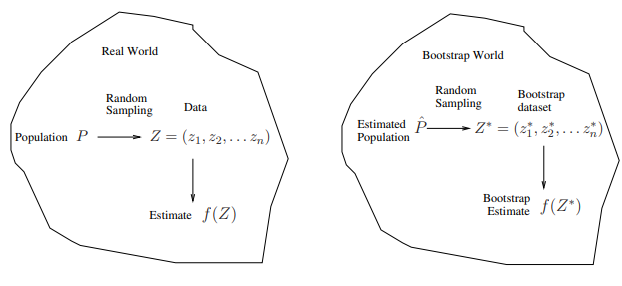
\includegraphics[width=1\textwidth,height=\textheight]{images/fromRealWorld2BootstrapWorld.png}

}

\end{figure}

\hypertarget{back-to-bagging}{%
\subsection{Back to bagging}\label{back-to-bagging}}

\begin{itemize}
\tightlist
\item
  Breiman (Breiman 1996) combined the ideas of:

  \begin{itemize}
  \tightlist
  \item
    Averaging provides decreased variance estimates,
  \item
    Bootstrap provides multiple (re)samples.
  \end{itemize}
\item
  He suggested: \textbf{b}ootstrap \textbf{agg}regat\textbf{ing} :

  \begin{itemize}
  \tightlist
  \item
    Take resamples from the original training dataset
  \item
    Learn the model on each bootstrapped training set to get a
    prediction \(\hat f^{*b}(x)\).
  \item
    Use the boostrap estimates to obtain improved
    prediction/classification.
  \end{itemize}
\end{itemize}

\hypertarget{bagging-predictionclassifier}{%
\subsection{Bagging
prediction/classifier}\label{bagging-predictionclassifier}}

\begin{itemize}
\tightlist
\item
  For regression (trees) the \textbf{bagged estimate} is the average
  prediction at \(x\) from these \(B\) trees.
\end{itemize}

\[\hat f_{bag}(x)=\frac 1B \sum_{b=1}^B \hat f^{*b}(x) \]

\begin{itemize}
\tightlist
\item
  For classification (trees) the \textbf{bagged classifier} selects the
  class with the most ``votes'' from the \(B\) trees:
\end{itemize}

\[
\hat G_{bag}(x) = \arg \max_k \hat f_{bag}(x).
\]

\hypertarget{out-of-bag-observations}{%
\subsection{Out-Of-Bag observations}\label{out-of-bag-observations}}

\begin{itemize}
\tightlist
\item
  Every time a resample is taken \emph{with replacement}, some
  observations are ommitted, due to the multiple occurring of others.
\end{itemize}

\begin{Shaded}
\begin{Highlighting}[]
\NormalTok{knitr}\SpecialCharTok{::}\FunctionTok{include\_graphics}\NormalTok{(}\StringTok{"images/oobErrorEstimation.jpg"}\NormalTok{)}
\end{Highlighting}
\end{Shaded}

\begin{figure}[H]

{\centering 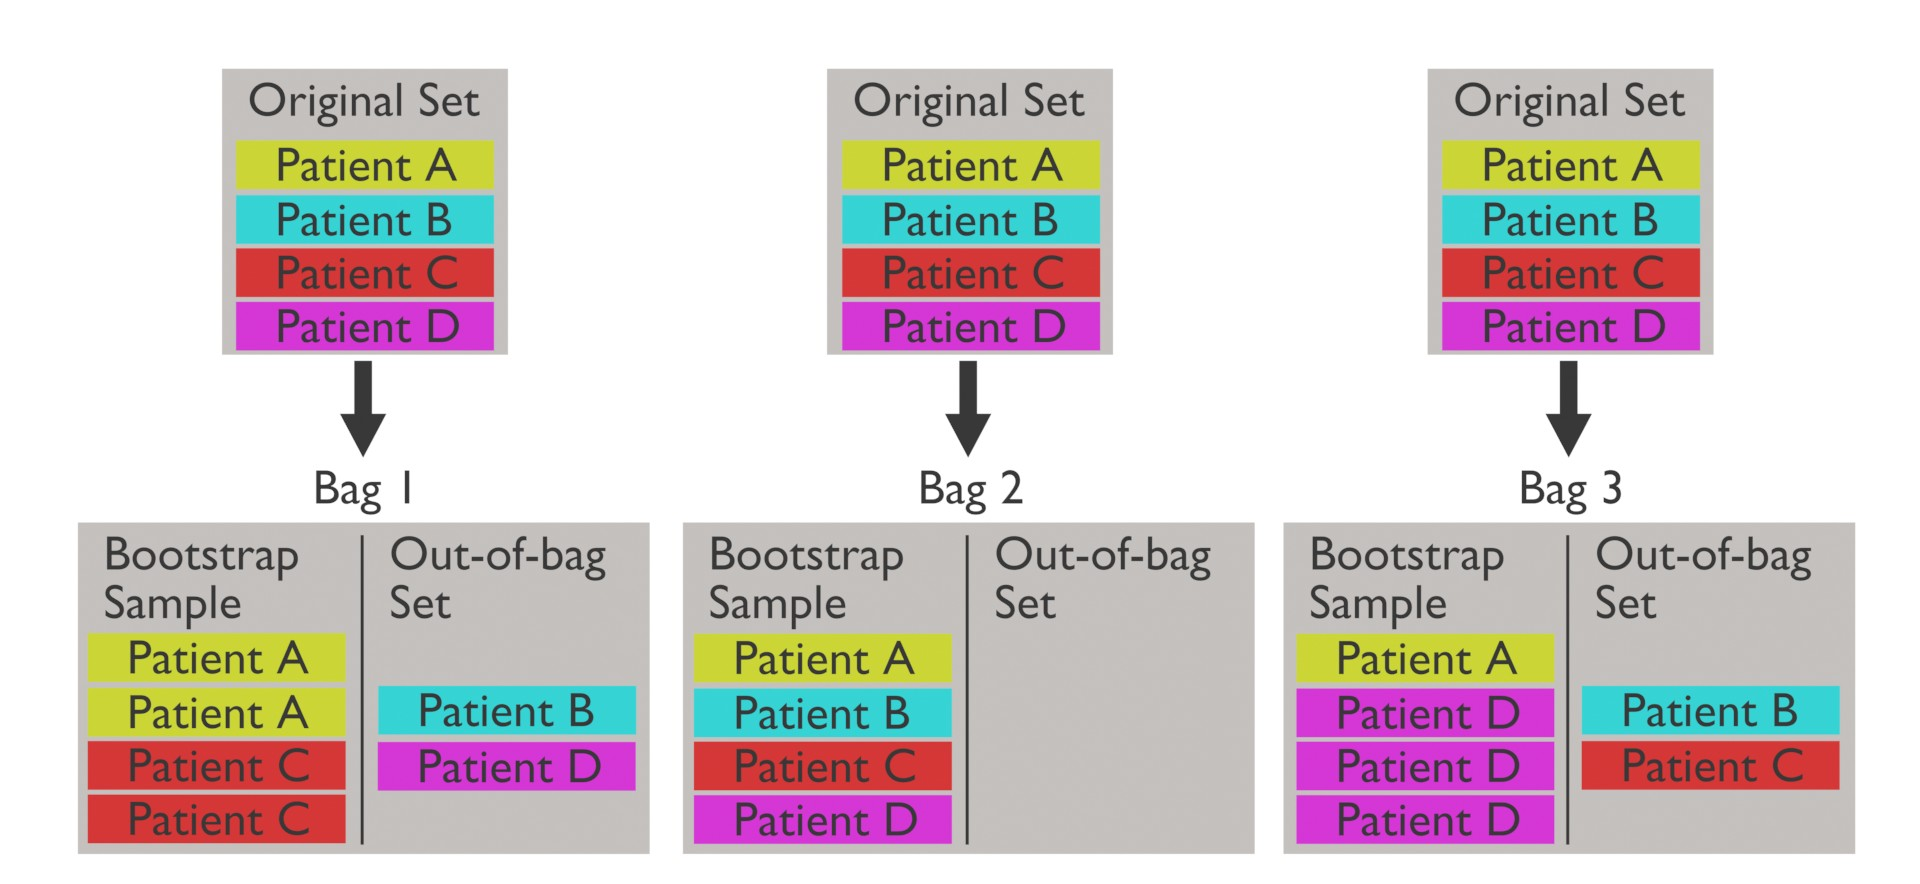
\includegraphics[width=1\textwidth,height=\textheight]{images/oobErrorEstimation.jpg}

}

\end{figure}

\begin{itemize}
\tightlist
\item
  These \emph{out-of-bag} (OOB) observations can be used to build an
  estimate of prediction error.
\end{itemize}

\hypertarget{out-of-bag-error-estimates}{%
\subsection{Out-Of-Bag error
estimates}\label{out-of-bag-error-estimates}}

Since each out-of-bag set is not used to train the model, it can be used
to evaluate performance.

\begin{enumerate}
\def\labelenumi{\arabic{enumi}.}
\tightlist
\item
  Find all trees that are not trained by the OOB instance.
\item
  Take the majority vote of these trees for the OOB instance, compared
  to the true value of the OOB instance.
\item
  Compile OOB error for all instances in the OOB dataset.
\end{enumerate}

\hypertarget{illustration-of-oob-ee}{%
\subsection{Illustration of OOB EE}\label{illustration-of-oob-ee}}

\begin{Shaded}
\begin{Highlighting}[]
\NormalTok{knitr}\SpecialCharTok{::}\FunctionTok{include\_graphics}\NormalTok{(}\StringTok{"images/oobErrorEstimation.png"}\NormalTok{)}
\end{Highlighting}
\end{Shaded}

\begin{figure}[H]

{\centering 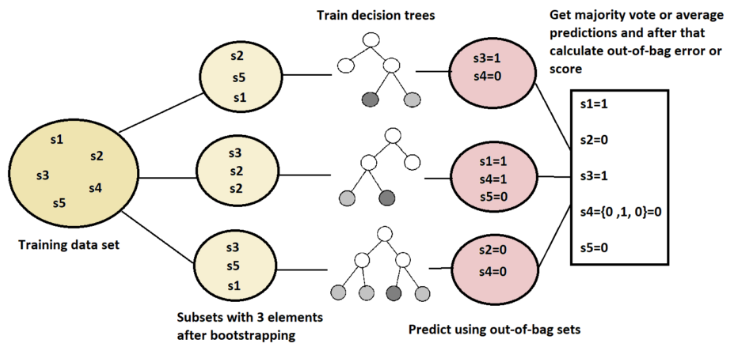
\includegraphics[width=1\textwidth,height=\textheight]{images/oobErrorEstimation.png}

}

\end{figure}

\href{https://www.baeldung.com/cs/random-forests-out-of-bag-error}{Source:
https://www.baeldung.com/cs/random-forests-out-of-bag-error}

\hypertarget{bagging-in-r-1.1}{%
\subsection{Bagging in R (1.1)}\label{bagging-in-r-1.1}}

\begin{itemize}
\item
  This exampe relies on the well-known \texttt{AmesHousing} dataset on
  house prices in Ames, IA.
\item
  We use libraries:

  \begin{itemize}
  \tightlist
  \item
    \texttt{rpart} for stratified resampling
  \item
    \texttt{ipred} for bagging.
  \end{itemize}
\end{itemize}

\begin{Shaded}
\begin{Highlighting}[]
\CommentTok{\# Prepare "clean" dataset from raw data}
\NormalTok{ames }\OtherTok{\textless{}{-}}\NormalTok{ AmesHousing}\SpecialCharTok{::}\FunctionTok{make\_ames}\NormalTok{()}

\CommentTok{\# Split in test/training}
\FunctionTok{set.seed}\NormalTok{(}\DecValTok{123}\NormalTok{)}
\NormalTok{split }\OtherTok{\textless{}{-}}\NormalTok{ rsample}\SpecialCharTok{::}\FunctionTok{initial\_split}\NormalTok{(ames, }\AttributeTok{prop =} \FloatTok{0.7}\NormalTok{, }
                       \AttributeTok{strata =} \StringTok{"Sale\_Price"}\NormalTok{)}
\NormalTok{ames\_train  }\OtherTok{\textless{}{-}} \FunctionTok{training}\NormalTok{(split)}
\NormalTok{ames\_test   }\OtherTok{\textless{}{-}} \FunctionTok{testing}\NormalTok{(split)}
\end{Highlighting}
\end{Shaded}

\hypertarget{bagging-in-r-1.2}{%
\subsection{Bagging in R (1.2)}\label{bagging-in-r-1.2}}

\begin{Shaded}
\begin{Highlighting}[]
\FunctionTok{system.time}\NormalTok{()}
\NormalTok{ames\_bag1 }\OtherTok{\textless{}{-}}\NormalTok{ ipred}\SpecialCharTok{::}\FunctionTok{bagging}\NormalTok{(}
  \AttributeTok{formula =}\NormalTok{ Sale\_Price }\SpecialCharTok{\textasciitilde{}}\NormalTok{ .,}
  \AttributeTok{data =}\NormalTok{ ames\_train,}
  \AttributeTok{nbagg =} \DecValTok{100}\NormalTok{,  }\AttributeTok{coob =} \ConstantTok{TRUE}\NormalTok{,}
  \AttributeTok{control =} \FunctionTok{rpart.control}\NormalTok{(}\AttributeTok{minsplit =} \DecValTok{2}\NormalTok{, }\AttributeTok{cp =} \DecValTok{0}\NormalTok{)}
\NormalTok{)}\ErrorTok{)}
\end{Highlighting}
\end{Shaded}

\begin{Shaded}
\begin{Highlighting}[]
\FunctionTok{show}\NormalTok{(ames\_bag1)}
\CommentTok{\# Bagging regression trees with 100 bootstrap replications }
\CommentTok{\# Call: bagging.data.frame(formula = Sale\_Price \textasciitilde{} ., data = ames\_train, }
\CommentTok{\#    nbagg = 100, coob = TRUE, control = rpart.control(minsplit = 2, }
\CommentTok{\#        cp = 0))}

\CommentTok{\# Out{-}of{-}bag estimate of root mean squared error:  26350.91 }
\end{Highlighting}
\end{Shaded}

\hypertarget{references}{%
\subsection*{References}\label{references}}
\addcontentsline{toc}{subsection}{References}

\hypertarget{refs}{}
\begin{CSLReferences}{1}{0}
\leavevmode\vadjust pre{\hypertarget{ref-Breiman1996}{}}%
Breiman, Leo. 1996. {``Bagging Predictors.''} \emph{Machine Learning}
24: 123--40. \url{https://doi.org/10.1007/BF00058655/METRICS}.

\leavevmode\vadjust pre{\hypertarget{ref-Efron79}{}}%
Efron, B. 1979. {``{Bootstrap Methods: Another Look at the
Jackknife}.''} \emph{The Annals of Statistics} 7 (1): 1--26.
\url{https://doi.org/10.1214/aos/1176344552}.

\end{CSLReferences}



\end{document}
